% Provenance (never printed): old premiere S material on the history of plate
% tectonics (from continental drift to seafloor spreading: the ridges, the
% magnetic stripes, the ages of the drilled floor); see
% sources/book2/PROVENANCE.md. Profiles are computed in
% figdata/grade-11/magnetic_stripes.py, the age map in seafloor_age.py, the
% drilling fit in sediment_ages.py.
\chapter{From Continental Drift to Seafloor Spreading}\label{ch:g11:drift-to-spreading}

In the early 1950s, at the Lamont laboratory of Columbia University, a young
geologist named Marie Tharp sat in front of long rows of numbers. Each was a depth of the North
Atlantic, measured by a ship's echo sounder, one after another along the ship's
track. Plotting them one by one, she drew the shape of the ocean floor along
the tracks of ships that had crossed the ocean. In the middle of the ocean the floor rose
into a mountain range --- and on every track, along the crest of the range, the
floor dropped again into a deep cleft, as if the mountains had been split down
the middle. This chapter follows how such measurements of the ocean floor turned
a rejected idea, the drift of the continents, into a theory: the ocean floor
is made at the ridges and spreads away from them, and it carries in its rocks a
record of its own age.
% ledger: aip:tharp, aip:featureless, usgs:echo-sounding

\begin{recall}
Continental drift is the idea that the continents move; Alfred Wegener
defended it from 1912 with the fit of the coasts, fossils, rocks and ancient
climates, but could not say what moved them. The surface of the Earth is made
of rigid plates, which meet at divergent, convergent and transform boundaries;
they move a few centimetres a year, and $\qty{1}{cm}$ a year is $\qty{10}{km}$
per million years (Book 1, grade 7). The ocean floor has its continental
shelf, its abyssal plains, its ridges and its trenches (Book 1, grade 8).
The Earth has a magnetic field, with a north and a south magnetic pole, that
a compass needle follows; a sound pulse sent into the water returns as an echo
after a time that gives the distance (the physics books).
\end{recall}

\section{Why drift was rejected}

Wegener's evidence showed that the continents had once been joined. What it
did not show was how they could have moved. Wegener imagined the continents
ploughing through the rock of the ocean floor, and physicists answered that no force known could push a continent through solid
rock without crushing it. For half a century most geologists concluded that
the continents had not moved at all.
% ledger: usgs:wegener-1912, usgs:jeffreys (Book 1 rows)

Two things were missing. The first was a mechanism. The second, which led to
the first, was knowledge of the floor of the oceans, which covers most of the
Earth's surface and which, in 1912, almost no one had seen: it was assumed to
be an almost featureless plain.
% ledger: aip:tharp, aip:featureless

\section{Mapping the ocean floor}

An echo sounder sends a short pulse of sound from the hull of a ship to the
sea floor and times its echo. Sound travels through sea water at about
\qty{1500}{m/s}; the pulse goes down and comes back, so a delay $t$ means a
depth
\[
  d = \frac{v\,t}{2}.
\]
A delay of \qty{6.0}{s}, for example, means $1500 \times 6.0/2 =
\qty{4500}{m}$ of water. In the nineteenth century, depths had been measured one
at a time, by lowering a weighted line to the bottom. After the First World
War, echo sounders took over, and the records of their echoes showed a floor
far more rugged than anyone had thought; in the 1950s surveys by ships of many nations showed that a
great mountain range on the ocean floor runs almost all the way around the
Earth.
% ledger: noaa:sound-seawater, usgs:echo-sounding, usgs:line-soundings

\begin{history}[Marie Tharp and the rift valley, 1952]
% ledger: aip:tharp, aip:featureless
From 1947, the geophysicist Bruce Heezen had gathered echo-sounding profiles
across the North Atlantic. Marie Tharp, who was not allowed on the research
ships at the time, turned what she later called ``interminable rows of
sounding numbers'' into drawings of the sea floor. By 1952, with the east--west
tracks arranged in order from north to south, she saw that one feature lined up
from track to track: a cleft along the crest of the Mid-Atlantic Ridge, a rift
valley. Heezen at first thought it was an error. Then the epicentres of the
earthquakes of the Atlantic, plotted at the same scale, were found to fall in
the rift valley itself. Tharp and Heezen's map of the world's ocean floor,
painted by the artist Heinrich Berann in 1977, gave people the first realistic picture of the ocean floor; in 1997 the
Library of Congress named her one of the four great cartographers of the
twentieth century.
\end{history}

The mid-ocean ridges form a single, nearly continuous system about
\qty{65000}{km} long, more than nine tenths of it under water; the crest lies
on average \qty{2500}{m} below the surface. Along the slow Mid-Atlantic Ridge,
the crest is cut by a rift valley; along the faster East Pacific Rise it is a
smooth, gentle summit. The earthquakes of the oceans follow the ridges
closely. Everything pointed to the ridge as a place
where something was happening --- but what?
% ledger: noaa:ridge, aip:tharp

\section{Seafloor spreading}

\begin{history}[Hess and the conveyor belt, 1962]
% ledger: usgs:hess, hess:1962
In 1962 Harry Hess, a geologist at Princeton University and an admiral of the
naval reserve, published \emph{History of Ocean Basins}.
He proposed that hot rock rises beneath the ridges and becomes new ocean floor,
which then moves away on both sides like a conveyor belt, and sinks back into
the mantle at the trenches. Robert Dietz, who reached the same idea, gave it
its name: \omterm{def:g11:drift-to-spreading:spreading}{seafloor spreading}. The idea explained why the Earth does not grow
although new floor is always being made, why so little sediment lies on the
ocean floor, and why the rocks of the ocean floor are much younger than those
of the continents.
\end{history}

\begin{definition}[Seafloor spreading]\label{def:g11:drift-to-spreading:spreading}
\emph{Seafloor spreading}\index{seafloor spreading} is the process by which
new ocean floor forms along the crest of a mid-ocean ridge, where molten rock
rises from the mantle and solidifies, and then moves away from the ridge on
both sides, so that the ocean floor grows older with distance from the ridge.
\end{definition}

\begin{definition}[Spreading rate]\label{def:g11:drift-to-spreading:spreading-rate}
The \emph{full spreading rate}\index{spreading rate} of a ridge is the speed at
which the two plates on either side of it move apart. The \emph{half spreading
rate} is the speed at which the floor on one side moves away from the ridge
axis. When spreading is symmetric, the full rate is twice the half rate.
\end{definition}

Ridges spread at very different speeds. The Mid-Atlantic Ridge opens at
\qtyrange{2}{5}{cm} a year, the East Pacific Rise at \qtyrange{6}{16}{cm} a
year. Of the ocean floor that exists today, about a third was made at slow
ridges (full rates of \qtyrange{20}{55}{mm} a year) and about two fifths at
fast ones (\qtyrange{75}{180}{mm} a year).
% ledger: noaa:ridge, seton:rate-classes

Hess's idea was bold, and at first it had little direct evidence. The evidence
came from two unexpected directions: the magnetism of the ocean floor and its
sediments.

\section{Magnetic reversals and the striped sea floor}

\subsection{A rock remembers the field}

The basalt of the ocean floor contains small grains of magnetite, an iron
oxide that is strongly magnetic. When basalt lava erupts, it is far too hot to
hold any lasting magnetisation; as it cools, the grains become magnetised
parallel to the Earth's field around them, and that direction is then locked
into the rock.
% ledger: usgs:magnetometers

\begin{definition}[Remanent magnetisation; Curie temperature]\label{def:g11:drift-to-spreading:remanence}
The \emph{Curie temperature}\index{Curie temperature} of a magnetic mineral is
the temperature above which it cannot keep a magnetisation of its own: about
\qty{580}{\celsius} for magnetite. A rock whose magnetic grains cool through
their Curie temperature in the Earth's field keeps a magnetisation parallel to
the field of that time, the \emph{remanent magnetisation}\index{remanent
magnetisation}. It lasts long after the field has changed, unless the rock is
heated again above the Curie temperature.
\end{definition}
% ledger: tarduno:curie

\begin{omfigure}
\begin{tikzpicture}[font=\footnotesize, >={Stealth[length=5pt]}]
  % ground and lava flow
  \fill[lith basalt] (0,0) rectangle (11,0.6);
  \fill[omLithBasalt!45!red!35] (0,0.6) -- (11,0.6) -- (11,1.9) .. controls (9,2.0) and (4,2.15) .. (0,2.05) -- cycle;
  \fill[omLithBasalt!70] (0,1.35) -- (11,1.25) -- (11,1.9) .. controls (9,2.0) and (4,2.15) .. (0,2.05) -- cycle;
  \draw[black!60] (0,1.35) -- (11,1.25);
  \draw[line width=0.8pt] (0,2.05) .. controls (4,2.15) and (9,2.0) .. (11,1.9);
  \draw[black!60] (0,0.6) -- (11,0.6);
  % field lines (northern hemisphere: pointing down to the north)
  \foreach \x in {0.6,2.4,4.2,6.0,7.8,9.6} {
    \draw[->, omDef, line width=0.9pt] (\x,4.0) -- (\x+1.1,2.55);
  }
  \node[anchor=south west, text=omDef] at (0.2,4.05) {the Earth's magnetic field};
  % locked grains in the cooled top
  \foreach \x in {0.5,1.3,...,10.5} {
    \draw[->, black, line width=0.6pt] (\x,1.86) -- (\x+0.25,1.53);
  }
  % random grains in the hot interior
  \foreach \x/\a in {0.6/20,1.5/140,2.3/250,3.2/80,4.0/310,4.9/190,5.7/40,6.6/120,7.4/280,8.3/20,9.1/200,10.0/330} {
    \draw[->, black!55, line width=0.5pt] (\x,0.95) -- ++(\a:0.22);
  }
  \node[anchor=west, align=left] at (11.15,1.75) {cooled below \qty{580}{\celsius}: the\\grains keep the field's direction};
  \node[anchor=west, align=left] at (11.15,0.92) {still above \qty{580}{\celsius}:\\no lasting magnetisation};
  \node[anchor=west, align=left] at (11.15,0.25) {older rock};
  \node[anchor=west] at (9.0,4.25) {north $\rightarrow$};
\end{tikzpicture}

{\small A lava flow cooling (schematic, Northern Hemisphere, where the field
points north and down). The top of the flow has cooled below the \omterm{def:g11:drift-to-spreading:remanence}{Curie
temperature} of magnetite: its magnetic grains (black arrows) keep the
direction of the field. The interior, still hotter, records nothing yet; it
will record the field of the moment it cools.}
\end{omfigure}

\subsection{The field reverses}

Early in the twentieth century, Bernard Brunhes (in 1906) and then Motonari
Matuyama (in the 1920s) found that volcanic rocks fall into two groups. In
some, the magnetisation points the way the present field does; in the others it
points the opposite way, as if the north and south magnetic poles had changed
places. The field itself had reversed, again and again.
% ledger: usgs:reversals

\begin{definition}[Magnetic reversal; normal and reversed polarity]\label{def:g11:drift-to-spreading:reversal}
A \emph{magnetic reversal}\index{magnetic reversal} is an exchange of the
Earth's north and south magnetic poles. A time when the field pointed as it
does today is a time of \emph{normal polarity}\index{normal polarity}; a time
when it pointed the opposite way, a time of \emph{reversed
polarity}\index{reversed polarity}. A rock magnetised during either time has
the same polarity.
\end{definition}

Dated lavas give the succession of normal and reversed intervals: the
\emph{geomagnetic polarity time scale}. Its long intervals are named after
scientists who studied the Earth's magnetism (Brunhes, Matuyama, Gauss,
Gilbert); the short events within them, after the places where they were
first found.

\begin{omfigure}
\begin{tikzpicture}
\begin{axis}[width=0.92\linewidth, height=3.2cm, xmin=0, xmax=5.5, ymin=-0.9, ymax=1.9,
  axis y line=none, axis x line*=bottom, xtick={0,0.5,...,5.5}, tick label style={font=\small},
  xlabel={age (million years)}, label style={font=\small}, clip=false]
\addplot[fill=black, draw=none] table {figdata/out/grade-11-magnetic_stripes-timescale.dat};
\draw[black] (axis cs:0,0) rectangle (axis cs:5.5,1);
\begin{scope}[every node/.style={font=\scriptsize, anchor=south}]
  \node at (axis cs:0.39,1.05) {Brunhes};
  \node at (axis cs:1.68,1.05) {Matuyama};
  \node at (axis cs:3.08,1.05) {Gauss};
  \node at (axis cs:4.74,1.05) {Gilbert};
\end{scope}
\draw[black!60] (axis cs:0.78,1) -- (axis cs:0.78,1.45);
\draw[black!60] (axis cs:2.581,1) -- (axis cs:2.581,1.45);
\draw[black!60] (axis cs:3.58,1) -- (axis cs:3.58,1.45);
\begin{scope}[every node/.style={font=\scriptsize, anchor=north}]
  \node at (axis cs:1.03,-0.05) {Jaramillo};
  \node at (axis cs:1.86,-0.05) {Olduvai};
\end{scope}
\node[font=\scriptsize, anchor=west] at (axis cs:5.55,0.75) {normal};
\node[font=\scriptsize, anchor=west] at (axis cs:5.55,0.25) {(black)};
\end{axis}
\end{tikzpicture}

{\small The geomagnetic polarity time scale for the last 5.5 million years:
black for \omterm{def:g11:drift-to-spreading:reversal}{normal polarity}, white for reversed. The present normal interval
began \num{780000} years ago; there were twenty reversals in the last five
million years. Data: Cande and Kent (1995).}
\end{omfigure}
% ledger: ck95:chrons

\subsection{Stripes on the ocean floor}

From the 1950s, ships towed magnetometers behind them across the oceans, and
found that the field at the sea surface was not the smooth field expected from
the Earth's core: it was a little stronger here, a little weaker there.
% ledger: usgs:magnetometers

\begin{definition}[Magnetic anomaly]\label{def:g11:drift-to-spreading:anomaly}
At a point of the sea surface, the \emph{magnetic anomaly}\index{magnetic
anomaly} is the measured strength of the magnetic field minus the strength
expected there from the Earth's field alone. It is positive where the rocks
below add to the field, negative where they oppose it. It is small compared
with the field itself, and measured in nanoteslas (\unit{nT}).
\end{definition}

Mapped over a wide region, the anomalies drew stripes parallel to the ridge
crest, alternately positive and negative, like a zebra's coat --- and the pattern
on one side of the ridge was the mirror image of the pattern on the other side.
% ledger: usgs:magnetometers

\begin{history}[Vine and Matthews, 1963]
% ledger: vm:1963, usgs:magnetometers
In September 1963, Fred Vine and Drummond Matthews published a short paper in the journal \emph{Nature},
\emph{Magnetic anomalies over oceanic ridges}. They put Hess's spreading and
the reversals of the field together. If new floor forms at the crest and moves
away while the field reverses, each strip of floor records the polarity of the
time when it cooled. The floor becomes a striped tape, unrolling on both sides
of the ridge: positive anomalies above normal strips, negative above reversed
ones, the same sequence on both sides.
\end{history}

\begin{omfigure}
\begin{tikzpicture}
\begin{axis}[hide axis, axis equal image, width=0.94\linewidth, xmin=-320, xmax=420, ymin=-120, ymax=160, clip=false]
  % block faces
  \fill[white] (axis cs:-300,0) -- (axis cs:300,0) -- (axis cs:390,70) -- (axis cs:-210,70) -- cycle;
  \fill[omLithBasalt!25] (axis cs:-300,0) rectangle (axis cs:300,-60);
  \fill[omLithBasalt!45] (axis cs:300,0) -- (axis cs:390,70) -- (axis cs:390,10) -- (axis cs:300,-60) -- cycle;
  \addplot[fill=black!80, draw=none] table {figdata/out/grade-11-magnetic_stripes-block.dat};
  \draw[black] (axis cs:-300,0) -- (axis cs:300,0) -- (axis cs:390,70) -- (axis cs:-210,70) -- cycle;
  \draw[black] (axis cs:-300,0) -- (axis cs:-300,-60) -- (axis cs:300,-60) -- (axis cs:300,0);
  \draw[black] (axis cs:300,-60) -- (axis cs:390,10) -- (axis cs:390,70);
  % ridge axis
  \draw[omRidge, line width=1.6pt] (axis cs:0,0) -- (axis cs:90,70);
  \node[font=\footnotesize, text=omRidge, anchor=south] at (axis cs:90,72) {ridge axis};
  % rising magma
  \fill[red!60!orange, opacity=0.75] (axis cs:-12,-60) -- (axis cs:12,-60) -- (axis cs:3,0) -- (axis cs:-3,0) -- cycle;
  \draw[->, >={Stealth[length=5pt]}, red!70!black, line width=1pt] (axis cs:0,-95) -- (axis cs:0,-62);
  \node[font=\footnotesize, anchor=north] at (axis cs:0,-96) {molten rock rises};
  % spreading arrows
  \draw[->, >={Stealth[length=6pt]}, line width=1.2pt] (axis cs:-90,100) -- (axis cs:-220,100);
  \draw[->, >={Stealth[length=6pt]}, line width=1.2pt] (axis cs:150,100) -- (axis cs:280,100);
  \node[font=\footnotesize, anchor=south] at (axis cs:-155,103) {older};
  \node[font=\footnotesize, anchor=south] at (axis cs:215,103) {older};
  % legend
  \fill[black!80] (axis cs:-300,-100) rectangle (axis cs:-280,-88);
  \node[font=\footnotesize, anchor=west] at (axis cs:-276,-94) {normal polarity};
  \draw[black] (axis cs:-300,-118) rectangle (axis cs:-280,-106);
  \node[font=\footnotesize, anchor=west] at (axis cs:-276,-112) {reversed polarity};
\end{axis}
\end{tikzpicture}

{\small The striped ocean floor (schematic, computed for a ridge spreading at
\qty{7.5}{cm} a year on each side, over the last 4 million years). Each strip
of floor kept the polarity of the field at the time it cooled at the axis;
the pattern on one side is the mirror image of the other.}
\end{omfigure}

\begin{proposition}[Distance of a stripe from the axis]\label{prop:g11:drift-to-spreading:stripe}
If a ridge spreads symmetrically at a constant half rate $u$, the floor that
formed at the axis a time $t$ ago now lies at a distance
\[
  x = u\,t
\]
on either side of the axis. In particular, the boundary between two stripes
that records a reversal of age $t$ lies at the distance $u\,t$ on both sides.
\end{proposition}

\begin{proof}
A piece of floor formed at the axis a time $t$ ago has since moved away from
the axis at the speed $u$, for the time $t$: it has covered the distance
$u\,t$. A piece formed at the same moment on the other side of the axis moves
the other way at the same speed, and lies at the same distance. The floor on
each side of a reversal boundary formed just before and just after the reversal,
so the boundary lies where floor of age $t$ lies: at $u\,t$.
\end{proof}

The anomalies can be computed from the time scale. In the profiles below, the
magnetised layer is a sheet of rock \qty{1}{km} thick whose top lies
\qty{3}{km} below the sea surface, divided into blocks of normal and \omterm{def:g11:drift-to-spreading:reversal}{reversed
polarity} by the proposition; the field of each block at the sea surface is
added up. Above a wide strip, the anomaly is strongest near its edges, where
the polarity changes, and weaker over its middle; but its sign follows the
polarity of the strip below.

\begin{omfigure}
\begin{tikzpicture}
\begin{axis}[omrecord, name=fast, width=0.92\linewidth, height=5.0cm, xmin=-375, xmax=375, ymin=-820, ymax=560,
  ytick={-400,0,400}, xtick={-300,-200,...,300}, tick label style={font=\small}, label style={font=\small},
  ylabel={anomaly (\unit{nT})}, title={\small fast ridge: half rate \qty{7.5}{cm} a year}, clip=false]
\addplot[fill=black, draw=none] table[y expr=\thisrow{y}*55-700] {figdata/out/grade-11-magnetic_stripes-fastblocks.dat};
\draw[black] (axis cs:-375,-755) rectangle (axis cs:375,-645);
\addplot[omDef, line width=0.9pt] table[x=x_km, y=anomaly_nT] {figdata/out/grade-11-magnetic_stripes-fast.dat};
\draw[black!40] (axis cs:-375,0) -- (axis cs:375,0);
\draw[black!50, densely dashed] (axis cs:268.5,-645) -- (axis cs:268.5,560);
\draw[black!50, densely dashed] (axis cs:-268.5,-645) -- (axis cs:-268.5,560);
\node[font=\scriptsize, anchor=south west, fill=white, inner sep=1pt] at (axis cs:270,-610) {3.58 million years};
\end{axis}
\begin{axis}[omrecord, at={(fast.south)}, anchor=north, yshift=-1.6cm, width=0.92\linewidth, height=5.0cm,
  xmin=-62.5, xmax=62.5, ymin=-820, ymax=560, ytick={-400,0,400}, xtick={-60,-40,...,60},
  tick label style={font=\small}, label style={font=\small},
  ylabel={anomaly (\unit{nT})}, xlabel={distance from the ridge axis (\unit{km})},
  title={\small slow ridge: half rate \qty{1.25}{cm} a year}, clip=false]
\addplot[fill=black, draw=none] table[y expr=\thisrow{y}*55-700] {figdata/out/grade-11-magnetic_stripes-slowblocks.dat};
\draw[black] (axis cs:-62.5,-755) rectangle (axis cs:62.5,-645);
\addplot[omProp, line width=0.9pt] table[x=x_km, y=anomaly_nT] {figdata/out/grade-11-magnetic_stripes-slow.dat};
\draw[black!40] (axis cs:-62.5,0) -- (axis cs:62.5,0);
\draw[black!50, densely dashed] (axis cs:44.75,-645) -- (axis cs:44.75,560);
\draw[black!50, densely dashed] (axis cs:-44.75,-645) -- (axis cs:-44.75,560);
\node[font=\scriptsize, anchor=south west, fill=white, inner sep=1pt] at (axis cs:45,-610) {3.58 million years};
\end{axis}
\end{tikzpicture}

{\small Magnetic anomalies computed across a fast and a slow ridge from the
polarity time scale, for floor up to 5 million years old on each side. Under
each profile, the strips of floor (black: normal; white: reversed). The
anomaly is positive above normal strips and negative above reversed ones; it
changes sign at the boundaries. The dashed lines mark the boundary of 3.58
million years. Note the different scales of distance: the slow ridge packs
the same history into a sixth of the width, and its shortest events blur
together. A model computed with chosen values (a layer magnetised at
\qty{5}{A/m}, magnetised vertically, as at high latitudes); time scale from
Cande and Kent (1995).}
\end{omfigure}
% values computed in figdata/grade-11/magnetic_stripes.py; ledger: ck95:chrons

\begin{method}[A spreading rate from a magnetic profile]\label{met:g11:drift-to-spreading:rate}
\begin{enumerate}
  \item Find the ridge axis: the centre of symmetry of the profile, in the
        middle of the central positive anomaly.
  \item Recognise a reversal boundary on both sides --- a sign change of the
        anomaly that the time scale dates --- and measure its distance from
        the axis on each side.
  \item Divide each distance by the age of the reversal: this gives the half
        rate on each side, in kilometres per million years
        ($\qty{10}{km}$ per million years is $\qty{1}{cm}$ a year).
  \item Add the two half rates to get the full rate.
\end{enumerate}
\end{method}

\begin{example}[The fast ridge]\label{ex:g11:drift-to-spreading:fast}
On the fast profile, the boundary between the Gauss and Gilbert intervals,
\num{3.58} million years old, lies \qty{268.5}{km} from the axis on each side.
The half rate is $268.5/3.58 = \qty{75}{km}$ per million years, that is
\qty{7.5}{cm} a year; the full rate is \qty{15}{cm} a year, the rate of the
fastest parts of the East Pacific Rise.
\end{example}
% values computed in figdata/grade-11/magnetic_stripes.py (fast_gg_km 268.5)

The magnetic stripes do more than confirm spreading: once a profile has been
matched to the time scale, every stripe gives the age of the floor beneath it.
In the 1960s, older stripes were dated by assuming a constant rate; a test of
the whole theory was to date the floor in a completely different way.
% ledger: whoi:h68

\section{Ages from the sediments}

Sediment --- the shells of tiny plankton, clay, dust --- settles slowly onto
the ocean floor and piles up over it. The oldest sediment lying directly on
the basalt was deposited soon after the basalt formed; its fossils, which
change from one age to the next, date it.

In 1968, the drilling ship \emph{Glomar Challenger}, built to drill into the
deep ocean floor and bring back cores, crossed the Mid-Atlantic Ridge between
South America and Africa. At seven sites along a line near latitude
\ang{30} South it drilled through the sediment into the basalt beneath, at
distances of \qty{191}{km} to \qty{1270}{km} from the ridge axis.
% ledger: usgs:glomar, dsdp3:rate, dsdp3:table5

\begin{omfigure}
\begin{tikzpicture}
\begin{axis}[omrecord, width=0.8\linewidth, height=6.2cm, xmin=0, xmax=1400, ymin=0, ymax=80,
  xlabel={distance from the ridge axis (\unit{km})}, ylabel={age (million years)},
  tick label style={font=\small}, label style={font=\small}, legend pos=north west,
  legend style={font=\scriptsize, cells={anchor=west}}]
\addplot[omProp, line width=0.9pt, domain=0:1400] table[x=dist_km, y=age] {figdata/out/grade-11-sediment_ages-fit.dat};
\addplot[only marks, mark=*, mark size=2pt, omDef, error bars/.cd, x dir=both, x explicit, y dir=both, y explicit]
  table[x=dist_km, y=age, x error=dist_err, y error=age_err] {figdata/out/grade-11-sediment_ages-sites.dat};
\addplot[only marks, mark=square, mark size=2.2pt, black] table[x=dist_km, y=age] {figdata/out/grade-11-sediment_ages-magnetic.dat};
\legend{{constant half rate \qty{1.9}{cm} a year}, {oldest sediment (fossils)}, {magnetic stripes}}
\node[font=\scriptsize, anchor=north west] at (axis cs:195,9.5) {16};
\node[font=\scriptsize, anchor=north west] at (axis cs:384,22.5) {15};
\node[font=\scriptsize, anchor=south east] at (axis cs:502,27) {18};
\node[font=\scriptsize, anchor=north west] at (axis cs:647,31.5) {17};
\node[font=\scriptsize, anchor=south east] at (axis cs:723,41) {14};
\node[font=\scriptsize, anchor=north west] at (axis cs:994,47.5) {19};
\node[font=\scriptsize, anchor=south east] at (axis cs:1266,68) {20};
\end{axis}
\end{tikzpicture}

{\small Age of the oldest sediment on the basalt at the seven drill sites of
1968 (numbered), against their distance from the axis of the Mid-Atlantic
Ridge; the squares give the ages of the magnetic stripes at the sites where
they were identified. The line is the constant half rate that fits the
sediment ages best. Data: Deep Sea Drilling Project, Leg 3 (1970).}
\end{omfigure}
% ledger: dsdp3:table5 (fit computed in figdata/grade-11/sediment_ages.py)

The ages grow steadily with distance from the ridge, on both sides of it: the
two sites drilled on the African side fall on the same line as those on the
American side. The best constant half rate is \qty{1.9}{cm} a year, and the
fossil ages agree with the ages predicted from the magnetic stripes. The
scientists of the expedition concluded that the floor had spread at a little
less than \qty{2}{cm} a year on each side for at least the last 66 million
years. \omterm{def:g11:drift-to-spreading:spreading}{Seafloor spreading} had passed a test it could have failed.
% ledger: dsdp3:rate, dsdp3:table5 (rate_palaeo_cm_yr 1.90 in figdata/grade-11/sediment_ages.py)

\begin{omfigure}
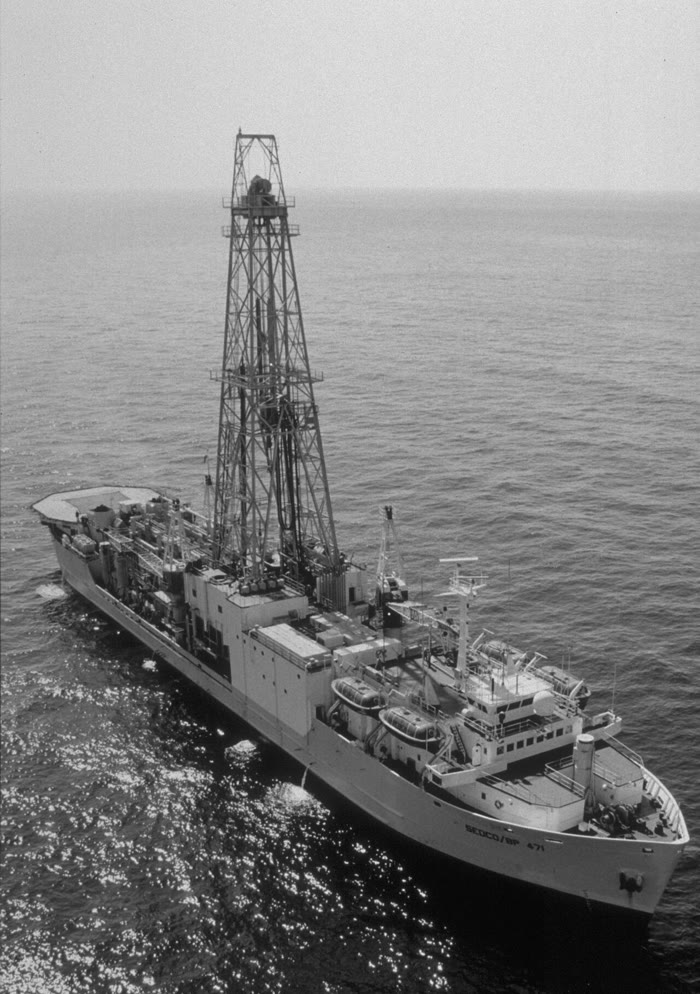
\includegraphics[width=0.36\linewidth]{images/book2/g11-odp-joides-resolution.jpg}

{\small The drilling ship \emph{JOIDES Resolution}, which succeeded the
\emph{Glomar Challenger}: the tall tower is its drilling derrick, and the
ship carries more than \qty{9000}{m} of drill pipe. Photograph: Ocean Drilling Program, Texas A\&M
University (public domain).}
\end{omfigure}
% ledger: photo:g11-joides, usgs:glomar

Since then, thousands of magnetic profiles and hundreds of drill holes have been
put together into a map of the age of the whole ocean floor.

\begin{omfigure}
\begin{tikzpicture}
\begin{axis}[ommap, width=\linewidth, xtick=\empty, ytick=\empty, grid=none,
    axis background/.style={}, clip=true, name=map]
  \addplot graphics[xmin=-180, xmax=180, ymin=-90, ymax=90] {figdata/out/grade-11-seafloor_age.png};
  \addplot[black!60, line width=0.15pt] table {figdata/out/shared-geo-land.dat};
\end{axis}
\begin{axis}[at={(map.south)}, anchor=north, yshift=-0.35cm, scale only axis, width=0.55\linewidth, height=0.32cm,
    xmin=0, xmax=200, ymin=0, ymax=1, axis y line=none, axis x line*=bottom,
    xtick={0,20,...,180}, tick label style={font=\scriptsize},
    xlabel={age of the ocean floor (million years); grey: no ocean floor}, label style={font=\scriptsize},
    enlargelimits=false]
  \addplot graphics[xmin=0, xmax=200, ymin=0, ymax=1] {figdata/out/grade-11-seafloor_age-bar.png};
\end{axis}
\end{tikzpicture}

{\small The age of the ocean floor. Youngest (red) along the ridges, it grows
older away from them on both sides; the oldest floor (blue and purple) lies
at the edges of the oceans, against the continents and along the trenches.
Data: Seton and others (2020), in 1-degree cells; land outlines: Natural
Earth.}
\end{omfigure}
% ledger: data:b2-seafloor-age, data:ne-land (map computed in figdata/grade-11/seafloor_age.py)

The map confirms everything at once. Along every ridge the floor is young,
and its age grows symmetrically away from it. No ocean floor is older than
about \num{190} million years: the oldest lies in the western Pacific and off
the east coast of North America (a few small basins of the eastern
Mediterranean are counted apart). The mean age of the ocean floor is about
\num{64} million years, and about three quarters of it is younger than 100
million years --- while the continents keep far older rocks. The
ocean floor is young because it is always being made at the ridges and, as
Hess saw, destroyed somewhere else: where, is the subject of
\cref{ch:g11:subduction-zones}.
% ledger: data:b2-seafloor-age (oldest_open_myr 192.5, share_younger_100 0.76 in figdata/grade-11/seafloor_age.py), seton:mean-age, usgs:hess

\section{Exercises}

\begin{exercise}[$\star$]\label{exo:g11:drift-to-spreading:1}
Define \omterm{def:g11:drift-to-spreading:spreading}{seafloor spreading}. What is the difference between the full and the
half \omterm{def:g11:drift-to-spreading:spreading-rate}{spreading rate} of a ridge?
\end{exercise}

\begin{exercise}[$\star$]\label{exo:g11:drift-to-spreading:2}
Why does a lava record the direction of the Earth's field only once it has
cooled below about \qty{580}{\celsius}? What happens to that record if the
rock is later heated to \qty{700}{\celsius}?
\end{exercise}

\begin{exercise}[$\star$]\label{exo:g11:drift-to-spreading:3}
An echo sounder hears the echo of its pulse \qty{5.2}{s} after sending it.
Taking the speed of sound in sea water as \qty{1500}{m/s}, how deep is the
sea floor?
\end{exercise}

\begin{exercise}[$\star$]\label{exo:g11:drift-to-spreading:4}
On the polarity time scale of this chapter: how long has the present normal
interval lasted? How long did the Jaramillo event last? How many reversals
happened in the last five million years?
\end{exercise}

\begin{exercise}[$\star$]\label{exo:g11:drift-to-spreading:5}
The mid-ocean ridges are about \qty{65000}{km} long. The circumference of the
Earth is about \qty{40000}{km}. How many times around the Earth would the
ridges go?
\end{exercise}

\begin{exercise}[$\star\star$]\label{exo:g11:drift-to-spreading:6}
On a magnetic profile, the boundary between the Brunhes and Matuyama intervals
(\num{0.78} million years) lies \qty{20}{km} from the ridge axis. Compute the
half rate and the full rate in centimetres a year.
\end{exercise}

\begin{exercise}[$\star\star$]\label{exo:g11:drift-to-spreading:7}
On another profile, the Gauss--Gilbert boundary (\num{3.58} million years) lies
\qty{45}{km} west and \qty{44}{km} east of the axis. Compute the half rate on
each side and the full rate. Is the spreading symmetric?
\end{exercise}

\begin{exercise}[$\star\star$]\label{exo:g11:drift-to-spreading:8}
Site 19 of the 1968 drilling lies \qty{990}{km} from the axis of the
Mid-Atlantic Ridge. Using a half rate of \qty{1.9}{cm} a year, predict the
age of the floor there, and compare with the \num{49} million years of its
oldest sediment.
\end{exercise}

\begin{exercise}[$\star\star$]\label{exo:g11:drift-to-spreading:9}
A ridge spreads at a half rate of \qty{2}{cm} a year. Using the time scale of
this chapter, give the distances from the axis of the boundaries at 0.78,
0.99, 1.07, 1.77 and 1.95 million years, and draw the stripes on one side,
normal in black.
\end{exercise}

\begin{exercise}[$\star\star$]\label{exo:g11:drift-to-spreading:10}
The mean age of the ocean floor is about \num{64} million years; the Earth is
about \num{4.6} billion years old. What fraction of the Earth's age is that?
Which of Hess's arguments does it support?
\end{exercise}

\begin{exercise}[$\star\star$]\label{exo:g11:drift-to-spreading:11}
Explain, with a drawing, why the pattern of magnetic stripes on one side of a
ridge is the mirror image of the pattern on the other side. What would break
this symmetry?
\end{exercise}

\begin{exercise}[$\star\star\star$]\label{exo:g11:drift-to-spreading:12}
Suppose the ridges, \qty{65000}{km} long in all, spread at an average full rate
of \qty{5}{cm} a year.
\begin{enumerate}
  \item What area of new ocean floor do they make each year, in \unit{km^2}?
  \item The ocean floor covers about \qty{2.9e8}{km^2}. How long would the
        ridges take to make that much?
  \item Compare with the oldest ocean floor, about \num{190} million years.
        What must happen to the ocean floor as fast as it is made?
\end{enumerate}
\end{exercise}

\begin{exercise}[$\star\star\star$]\label{exo:g11:drift-to-spreading:13}
The Jaramillo event lasted from \num{0.99} to \num{1.07} million years ago.
How wide is its stripe on each side of a ridge with a half rate of
\qty{1.25}{cm} a year, and of one with \qty{7.5}{cm} a year? The magnetised
rock lies about \qty{3}{km} below the sea surface. Explain why the event shows
clearly on the fast profile of this chapter but hardly at all on the slow one.
\end{exercise}

\begin{exercise}[$\star\star\star$]\label{exo:g11:drift-to-spreading:14}
At the 1968 sites, the sediment is \qty{176}{m} thick at site 16, whose floor
is about \num{11} million years old, and only \qty{72}{m} thick at site 20,
about \num{67} million years old. Compute the average rate at which sediment
piled up at each site, in metres per million years. Can the thickness of the
sediment be used to date the floor? What is used instead?
\end{exercise}

\begin{exercise}[$\star\star\star$]\label{exo:g11:drift-to-spreading:15}
On a profile across a ridge, the boundary of \num{2.581} million years lies
\qty{58}{km} west and \qty{70}{km} east of the axis.
\begin{enumerate}
  \item Compute the half rate on each side and the full rate.
  \item The floor east of the axis was made faster than the floor west of it.
        After 10 million years at these rates, how far from the axis would
        floor of that age lie on each side?
  \item Explain why the distance between the two boundaries gives the full
        rate even if the spreading is not symmetric.
\end{enumerate}
\end{exercise}

\section{Problem: The Age of the South Atlantic}

\begin{problem}[{Weekend problem --- dating an ocean in three ways}]
\label{pb:g11:drift-to-spreading:1}
% ledger: dsdp3:table5, dsdp3:rate, data:b2-seafloor-age, earth:Rmean, ics:base.Cretaceous
% (values computed in figdata/grade-11/sediment_ages.py and seafloor_age.py)
In 1968 the \emph{Glomar Challenger} drilled seven holes across the
Mid-Atlantic Ridge near latitude \ang{30} South. The table gives, for each
site, its distance from the ridge axis, the age of the oldest sediment on the
basalt (from its fossils) and, where the stripe beneath it was identified, the
age of that magnetic stripe, in millions of years.

\begin{center}
\small
\begin{tabular}{|c|c|c|c|}
\hline
site & distance from the axis (\unit{km}) & age of the oldest sediment & age of the magnetic stripe \\ \hline
16 & 191 & 11 & 9 \\ \hline
15 & 380 & 24 & 21 \\ \hline
18 & 506 & 26 & --- \\ \hline
17 & 643 & 33 & --- \\ \hline
14 & 727 & 40 & 38.5 \\ \hline
19 & 990 & 49 & 53 \\ \hline
20 & 1270 & 67 & 71 \\ \hline
\end{tabular}

{\small Data: Deep Sea Drilling Project, Leg 3 (1970); magnetic ages are the
middle of the ranges given there.}
\end{center}

\begin{center}
\begin{tikzpicture}
\begin{axis}[omrecord, width=0.82\linewidth, height=5.0cm, xmin=-50, xmax=16, ymin=0, ymax=140,
  xlabel={longitude along \ang{30} South (degrees; negative: west)}, ylabel={age (million years)},
  tick label style={font=\small}, label style={font=\small}, clip=false]
\addplot[omDef, line width=0.8pt] table[x=lon, y=age] {figdata/out/grade-11-seafloor_age-profile.dat};
\draw[omRidge, densely dashed] (axis cs:-13.8,0) -- (axis cs:-13.8,140);
\node[font=\scriptsize, text=omRidge, anchor=south] at (axis cs:-13.8,140) {ridge axis};
\fill (axis cs:-47.4,125.1) circle (1.5pt);
\node[font=\scriptsize, anchor=south west, inner sep=2pt] at (axis cs:-47.6,126) {South America};
\node[font=\scriptsize, anchor=north west, align=left] at (axis cs:14.2,135) {Africa};
\fill (axis cs:13.8,129.8) circle (1.5pt);
\end{axis}
\end{tikzpicture}

{\small The age of the ocean floor along the parallel \ang{30} South, from
South America to Africa; the line stops where the ocean floor ends against
each continent. Data: Seton and others (2020).}
\end{center}

\medskip
\noindent\textbf{Part I --- The drill sites.}
\begin{enumerate}
  \item Which site lies closest to the ridge, and which farthest? How do
        their ages compare?
  \item Why is the age of the oldest sediment lying on the basalt close to
        the age of the basalt itself? Is it a little older or a little
        younger?
  \item For each site, compute the ratio of its distance to the age of its
        oldest sediment, in kilometres per million years.
  \item What is the mean of these seven ratios? Convert it to centimetres a
        year.
  \item Sites 17 and 18 lie east of the ridge, the others west of it. Do the
        eastern sites follow the same trend as the western ones? What does
        that say about the spreading?
\end{enumerate}

\medskip
\noindent\textbf{Part II --- The rate from the sediments.}
\begin{enumerate}[resume]
  \item If the floor spread at a constant half rate $u$, how would the age
        $t$ of the floor depend on its distance $d$ from the axis?
  \item The line through the origin that fits the points best has the slope
        $u = \sum d\,t / \sum t^2$. For the seven sites,
        $\sum d\,t = \num{208276}$ and $\sum t^2 = \num{10952}$ (in
        kilometres and millions of years). Compute $u$ in kilometres per
        million years and in centimetres a year.
  \item What is the \omterm{def:g11:drift-to-spreading:spreading-rate}{full spreading rate} of the South Atlantic at this
        latitude?
  \item The expedition's scientists wrote that the rate was ``slightly less
        than \qty{2}{cm} a year''. Do you agree?
  \item With this rate, predict the age of the floor at site 20, and compare
        with its oldest sediment.
\end{enumerate}

\medskip
\noindent\textbf{Part III --- The rate from the magnetic stripes.}
\begin{enumerate}[resume]
  \item From site 16 alone (\qty{191}{km}, stripe of 9 million years),
        compute a half rate.
  \item From site 20 alone (\qty{1270}{km}, stripe of 71 million years),
        compute a half rate.
  \item For the five sites with a magnetic age, $\sum d\,t = \num{180329}$ and
        $\sum t^2 = \num{9854}$. Compute the best half rate.
  \item By how many per cent do the rates from the fossils and from the
        stripes differ? Do the two methods agree?
  \item Why is it important that the two ages were found by completely
        different methods?
\end{enumerate}

\medskip
\noindent\textbf{Part IV --- To the edge of the ocean.}
\begin{enumerate}[resume]
  \item Along \ang{30} South, the ridge axis lies at longitude
        \ang{13.8} West and the ocean floor ends against Africa at
        \ang{13.8} East. How many degrees of longitude separate them?
  \item On a sphere of radius \qty{6371}{km}, one degree of longitude
        measures $\qty{111.2}{km} \times \cos(\text{latitude})$. Compute the
        length of one degree at \ang{30} South, and the distance from the
        axis to the edge of the ocean floor beside Africa.
  \item If the floor had always spread at the rate of Part II, how long ago
        would the floor at the edge have formed?
  \item The age map, which dates the old floor by its magnetic stripes, gives
        \num{130} million years at the edge. What average half rate does
        that imply? Was the early opening of the ocean a little faster or a
        little slower than the opening of the last 66 million years?
  \item Conclude: how old is the oldest ocean floor beside Africa at
        \ang{30} South? The Cretaceous period began about \num{143} million
        years ago: in which period did the South Atlantic begin to open
        there?
\end{enumerate}
\end{problem}
